\chapter{Objetivo}

\nocite{statistics}
\nocite{irms}
\nocite{forbes}

\capepigrafe[0.5\textwidth]{First to mind when asked what 'the cloud' is, a majority respond it’s either an actual cloud, the sky, or something related to weather.}{Citrix Cloud Survey Guide\cite{quotes}}

Com o desenvolvimento da computação, novos programas foram criados, cada vez mais consumindo recursos e sendo hospedados em máquinas pessoais ou dedicadas, porém sem um gerenciamento inteligente de toda a infraestrutura. Além disso, houve a nítida migração de programas \textbf{distribuídos} pela internet para programas que \textbf{rodem} na internet.

\begin{figure}[h!]
  \centering
  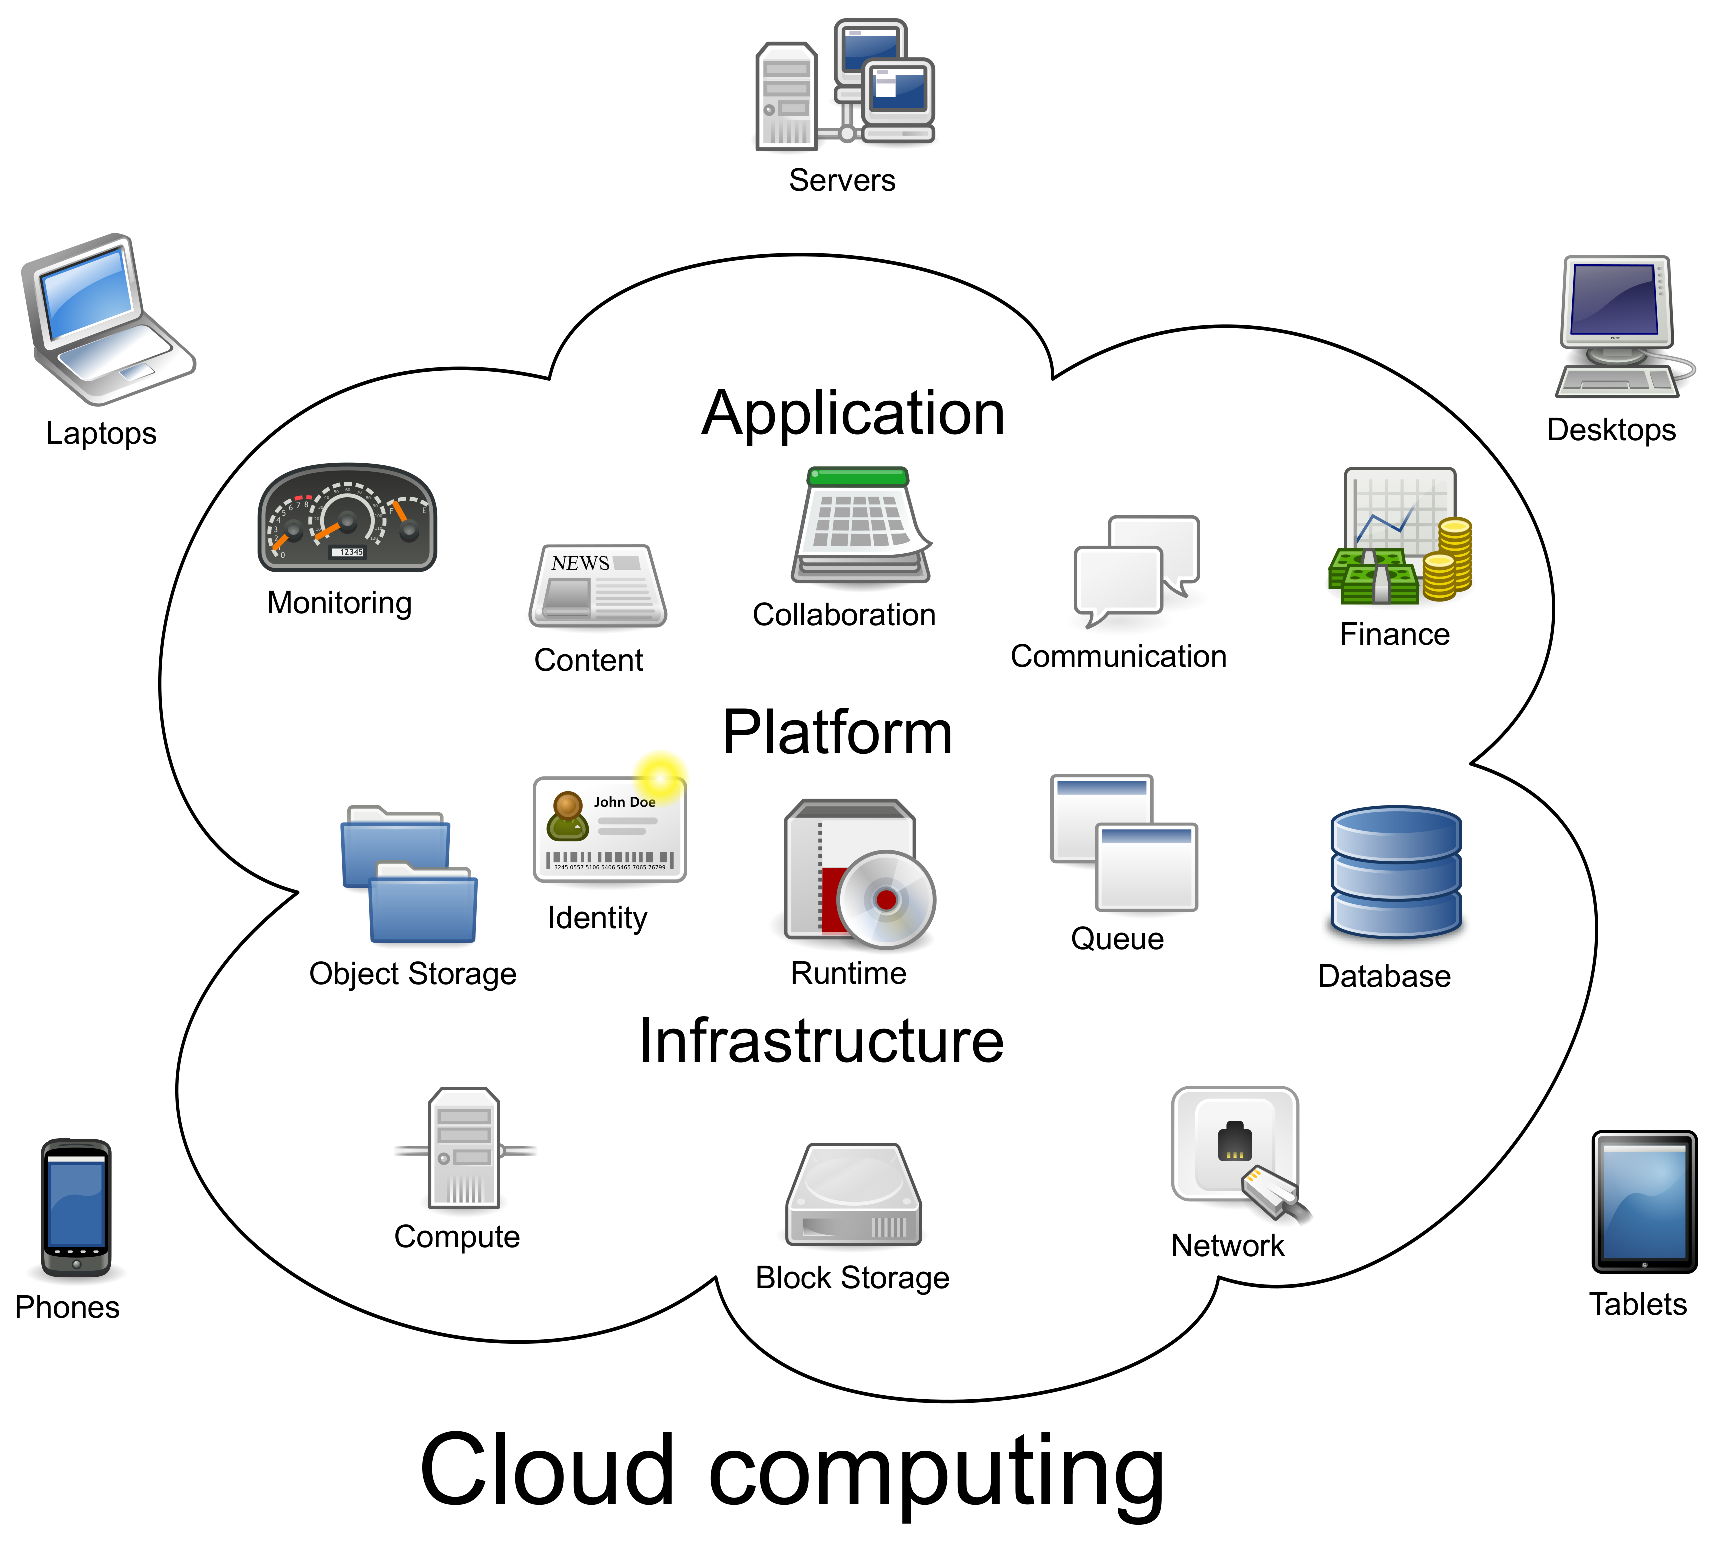
\includegraphics[scale=0.40]{imagens/cloud_computing.eps}
  \caption{Arquitetura Básica de Computação em Nuvem\cite{cloudcomputing}}
\end{figure}

Essas mudanças de paradigma motivaram a criação e consolidação do que conhecemos hoje como Computação em Nuvem, área fortalecida e necessária no desenvolvimento de programas modernos. Ao longo dos pŕoximos capítulos, haverá a explanação em detalhes de como funciona uma arquitetura em nuvem básica, seus desafios técnicos e as principais soluções existentes no mercado.
